Una volta identificati i cerchi di iride e pupilla e salvati i relativi parametri di centro e raggio in due vettori, rispettivamente chiamati \texttt{iris\_circle} e \texttt{pupil\_circle}, si passa alla segmentazione vera e propria, nella quale viene isolata la regione di interesse dell’iride. A tale scopo è stata definita una funzione all’interno di \texttt{processing.py} denominata segmentation:

\begin{minted}
  [
    xleftmargin=\parindent,
    framesep=2mm,
    baselinestretch=1.2,  
    fontsize=\footnotesize,
    linenos,
    breaklines
  ]
  {python}
  
  def segmentation(image, iris_circle, pupil_circle, startangle, endangle, min_radius, max_radius)  
\end{minted}

La funzione prende in input i vettori dei parametri dei cerchi, \texttt{iris\_circle} e \texttt{pupil\_circle}, un angolo di partenza, uno di fine e due valori limite di raggio. Per adattare il codice ad ogni tipo di dimensione si è utilizzato un approccio particolare, basato sull’uso di percentuali. In questo modo è possibile ottenere porzioni intermedie di iride indicando la percentuale minima e massima del raggio totale che si vuole considerare. I valori percentuali di default sono 0\% e 100\% in modo da prendere l’intera iride, quindi partendo dal bordo della pupilla (identificato dal suo raggio) ed arrivando fino al bordo esterno, tuttavia risultano modificabili tramite i parametri \texttt{MIN\_RADIUS} e \texttt{MAX\_RADIUS} della sezione \texttt{PREPROCESSING} del file di configurazione. Nel caso di inserimento di valori fuori limite verranno in automatico utilizzati i valori di default.

\begin{minted}
  [
    xleftmargin=\parindent,
    framesep=2mm,
    baselinestretch=1.2,  
    fontsize=\footnotesize,
    linenos,
    breaklines
  ]
  {python}
  
  outer_sector = np.zeros((height, width), np.uint8)
  inner_sector = np.zeros((height, width), np.uint8)

  if min_radius < max_radius:
      draw_ellipse(outer_sector, (iris_circle[0], iris_circle[1]), (
          max_radius, max_radius), 0, -startangle, -endangle, 255, thickness=-1)
      cv2.circle(inner_sector, (pupil_circle[0], pupil_circle[1]), int(
          min_radius), 255, thickness=-1)
  mask = cv2.subtract(outer_sector, inner_sector)
  masked_image = cv2.bitwise_and(segmented, segmented, mask=mask)

  return masked_image, mask 
\end{minted}

Il funzionamento è semplice: si inizializzano delle maschere, rappresentate da delle matrici di zeri della stessa dimensione dell’immagine originale (immagini nere), in questo caso chiamate \texttt{outer\_sector} e \texttt{inner\_sector}. Le maschere sono un modo per selezionare parti specifiche di immagini, in sostanza si vanno a marcare i pixel che si vogliono considerare mettendo a 1 i valori nelle rispettive posizioni nella maschera. Facendo l’AND logico tra la maschera e l’immagine originale si ottengono solo i pixel corrispondenti alla parte desiderata dell’immagine. Si utilizzano quindi i parametri di \texttt{iris\_circle} e \texttt{pupil\_circle} e quelli definiti dall’utente nella chiamata alla funzione per creare due maschere. La prima consiste in un settore circolare con raggio uguale al raggio massimo definito precedentemente. Essa viene ottenuta grazie alla funzione \texttt{draw\_ellipse}, si crea poi la seconda maschera, corrispondente ad un cerchio di raggio minimo (se 0\% il cerchio corrisponde alla pupilla) tramite la funzione \texttt{cv2.circle}. Successivamente, tramite la funzione di OpenCV \texttt{cv2.subtract} si crea un’unica maschera finale contenente i pixel ottenuti dalla dalla sottrazione tra \texttt{outer\_sector} e \texttt{inner\_sector}, ottenendo così la maschera relativa all’area di interesse. Infine l’area di interesse vera e propria è ricavata tramite la funzione \texttt{cv2.bitwise\_and}, la quale effettua una AND tra l’immagine di partenza e l’ultima  maschera creata, ottenendo così i soli pixel reali del segmento di iride.

\begin{figure}[h]
  \centering
  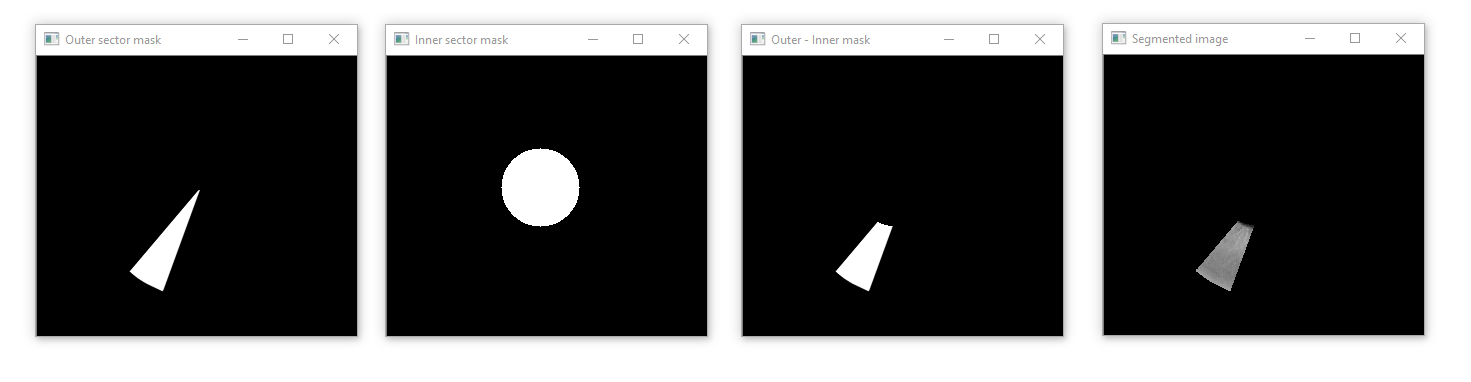
\includegraphics[width=1.0\textwidth]{segmentazione.png}
  \caption{Segmentazione dell'iride per ottenere la regione d'interesse}
\end{figure}
